\documentclass[11pt,a4paper]{article}
\usepackage[margin=2.3cm]{geometry}
\usepackage[T1]{fontenc}
\usepackage{textcomp}
\input{glyphtounicode}
\pdfgentounicode=1
\usepackage{lmodern}
\usepackage{amsmath}
\usepackage{xcolor}
\usepackage{listings}
\usepackage{tcolorbox}
\tcbuselibrary{breakable}
\usepackage{booktabs}
\usepackage{array}
\usepackage{tikz}
\usetikzlibrary{decorations.pathreplacing}
\usepackage{float}
\usepackage{graphicx}
\graphicspath{{images/}}
\usepackage{hyperref}
\hypersetup{colorlinks=true, linkcolor=blue!50!black, citecolor=green!40!black}

\usepackage{accsupp}
% line numbers are drawn but excluded from copied text
\newcommand{\nocopy}[1]{\BeginAccSupp{method=escape,ActualText={}}#1\EndAccSupp{}}
\lstset{
  language=C, basicstyle=\ttfamily\small, keywordstyle={}, commentstyle={}, stringstyle={},
  numbers=left, numberstyle=\footnotesize\nocopy, numbersep=10pt, xleftmargin=2.4em,
  frame=none, columns=fullflexible, keepspaces=true, upquote=true, showstringspaces=false,
  breaklines=true, captionpos=b, aboveskip=1em, belowskip=0.8em
}
\lstdefinestyle{sh}{language=bash, numbers=none, xleftmargin=2.4em}
\renewcommand{\lstlistingname}{Listing}
% code names in the text: grey monospace
\let\origtexttt\texttt
\renewcommand{\texttt}[1]{\textcolor{black!60}{\origtexttt{#1}}}

\newtcolorbox{keyidea}{colback=blue!4, colframe=blue!45!black, title=Key ideas, fonttitle=\bfseries\small}
\newtcolorbox{experiment}{breakable, colback=orange!5, colframe=orange!70!black, title=Experiment, fonttitle=\bfseries\small}
\title{\textbf{OpenMP GPU Data: \texttt{target enter data}, \texttt{exit data} and \texttt{update}}\\[4pt]\large Lesson 31: keeping data on the GPU and reading only what you need}
\author{Gustavo Lozano}
\date{November 2026}

\begin{document}
\maketitle

\noindent\textit{\small Source: Deakin \& Mattson~\cite{dm}, Ch.~4 (Memory Movement).
Prerequisite: \texttt{00-openmp\_target.pdf} (Lesson 30).}

\section{The idea}
Lesson 30 showed that the PCIe bus is the slowest link: data should go to the GPU once and stay
there. A \texttt{target data} region does that, but only inside one block of code. Real
programs allocate in one function, compute in others and free at the end, and they need to
look at results while the data stays on the GPU. Three constructs do this:

\begin{center}
\small
\begin{tabular}{@{}lp{8.9cm}@{}}
\toprule
construct & effect \\ \midrule
\texttt{target enter data map(to: a[0:n])} & allocate \texttt{a} on the device and copy it
there; it stays until \texttt{exit data} \\
\texttt{target exit data map(from: a[0:n])} & copy \texttt{a} back and free it on the device \\
\texttt{target exit data map(delete: a[0:n])} & free it without copying \\
\texttt{target update from(a[i:k])} & copy $k$ elements device $\rightarrow$ host; the data
stays \\
\texttt{target update to(a[i:k])} & copy $k$ elements host $\rightarrow$ device \\
\bottomrule
\end{tabular}
\end{center}

Between \texttt{enter data} and \texttt{exit data} the array is \emph{present} on the device.
A \texttt{target} region that maps it copies nothing. Writing
\texttt{map(present, alloc: a[0:n])} says so explicitly: the program stops with an error if
\texttt{a} is not on the device, instead of copying it silently.

\begin{figure}[H]
\centering
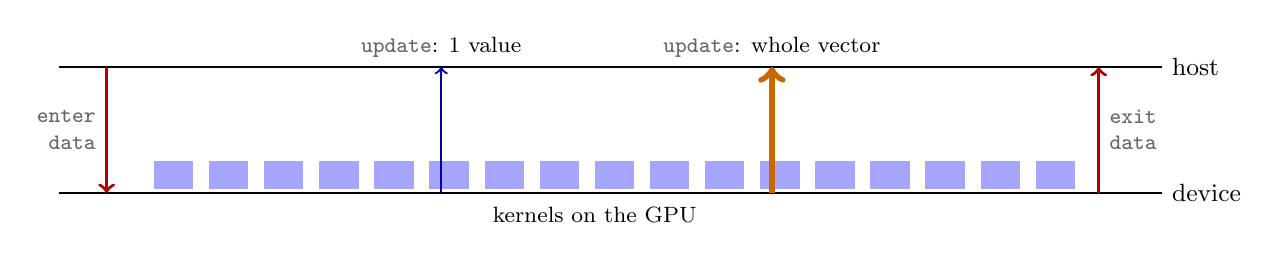
\begin{tikzpicture}[font=\small, x=1cm, y=1cm]
  \draw[thick] (0,1.6) -- (14,1.6) node[right] {host};
  \draw[thick] (0,0) -- (14,0) node[right] {device};
  \draw[->, very thick, red!70!black] (0.6,1.6) -- (0.6,0) node[midway, left, align=right,
     font=\footnotesize] {\texttt{enter}\\\texttt{data}};
  \foreach \x in {1.2,1.9,...,12.4} \fill[blue!35] (\x,0.05) rectangle ++(0.5,0.35);
  \node[below, font=\footnotesize] at (6.8,-0.05) {kernels on the GPU};
  \draw[->, thick, blue!70!black] (4.85,0) -- (4.85,1.6);
  \node[above, font=\footnotesize, align=center] at (4.85,1.6) {\texttt{update}: 1 value};
  \draw[->, line width=2.4pt, orange!80!black] (9.05,0) -- (9.05,1.6);
  \node[above, font=\footnotesize, align=center] at (9.05,1.6) {\texttt{update}: whole vector};
  \draw[->, very thick, red!70!black] (13.2,0) -- (13.2,1.6) node[midway, right, align=left,
     font=\footnotesize] {\texttt{exit}\\\texttt{data}};
\end{tikzpicture}
\caption{The vector crosses the bus once in each direction (\texttt{enter}/\texttt{exit data}).
In between, \texttt{target update} copies only the section it names.}
\label{fig:life}
\end{figure}

\section{The example}
A vector \texttt{x} of $2^{25}$ doubles (256\,MiB) goes to the GPU once. A kernel adds 1 to every
element, 200 times; every 10 steps the host looks at \texttt{x}.
\begin{itemize}
  \item \texttt{to\_device} and \texttt{from\_device} (lines 23--31) open and close the life of
        \texttt{x} on the GPU. They are separate functions, which \texttt{target data} cannot do.
  \item \texttt{add\_one} (lines 34--39) requires \texttt{x} to be present and copies nothing.
  \item The host reads nothing, only \texttt{x[0:1]} (line 51), or all of \texttt{x[0:n]}
        (line 53).
\end{itemize}
At the end every element must be 200.

\begin{lstlisting}[caption={\textbf{\origtexttt{target\_update.c}} -- a vector kept on the GPU and read with \origtexttt{target update}.}, label={lst:upd}]
/*
 * target_update.c -- OpenMP Lesson 31: data that lives on the GPU,
 * with target enter data, target exit data and target update.
 * Source: Deakin & Mattson (2023), Ch. 4 (Memory Movement).
 *
 * A vector x stays on the GPU while a kernel adds 1 to every element NSTEP
 * times.  Every EVERY steps the host looks at x: not at all, only x[0],
 * or the whole vector.
 *
 * Compile:  clang -O2 -fopenmp --offload-arch=sm_61 \
 *                 -o target_update target_update.c
 * Run:      OMP_TARGET_OFFLOAD=MANDATORY ./target_update [log2 n]
 */

#include <stdio.h>
#include <stdlib.h>
#include <omp.h>

#define NSTEP 200
#define EVERY 10

/* ---- data lifetime on the device -------------------------------------- */
static void to_device(double *x, long n)
{
    #pragma omp target enter data map(to: x[0:n])      /* allocate + copy in */
}

static void from_device(double *x, long n)
{
    #pragma omp target exit data map(from: x[0:n])     /* copy out + free    */
}

/* ---- the kernel: x must already be on the device ---------------------- */
static void add_one(double *x, long n)
{
    #pragma omp target teams distribute parallel for map(present, alloc: x[0:n])
    for (long i = 0; i < n; i++)
        x[i] += 1.0;
}

/* NSTEP kernels; mode 0: no reads, 1: read x[0], 2: read all of x */
static double run(double *x, long n, int mode)
{
    for (long i = 0; i < n; i++) x[i] = 0.0;
    double t = omp_get_wtime();
    to_device(x, n);
    for (int k = 1; k <= NSTEP; k++) {
        add_one(x, n);
        if (k % EVERY == 0) {
            if (mode == 1) {
                #pragma omp target update from(x[0:1])
            } else if (mode == 2) {
                #pragma omp target update from(x[0:n])
            }
        }
    }
    from_device(x, n);
    return omp_get_wtime() - t;
}

static const char *check(const double *x, long n)
{
    for (long i = 0; i < n; i++)
        if (x[i] != NSTEP) return "NO";
    return "yes";
}

int main(int argc, char **argv)
{
    long n = 1L << (argc > 1 ? atoi(argv[1]) : 25);   /* 2^25 doubles = 256 MiB */
    double *x = malloc(n * sizeof(double));

    int on_host = 1;                                  /* also starts up the GPU */
    #pragma omp target map(from: on_host)
    on_host = omp_is_initial_device();
    printf("ran on: %s, n = %ld (%.0f MiB), %d steps, reads every %d\n",
           on_host ? "CPU" : "GPU", n, n * 8.0 / (1 << 20), NSTEP, EVERY);

    const char *name[3] = {"no reads", "read x[0]", "read all x"};
    for (int mode = 0; mode < 3; mode++) {
        double t = run(x, n, mode);
        printf("%-11s: %6.3f s   correct: %s\n", name[mode], t, check(x, n));
    }
    free(x);
    return 0;
}
\end{lstlisting}

\begin{lstlisting}[style=sh]
clang -O2 -fopenmp --offload-arch=sm_61 -o target_update target_update.c
OMP_TARGET_OFFLOAD=MANDATORY ./target_update
\end{lstlisting}

\begin{keyidea}
\begin{itemize}
  \item \texttt{target enter data} / \texttt{exit data}: the data lives on the GPU from one
        call to another, across functions.
  \item \texttt{map(present, alloc: ...)}: use data that must already be on the device.
  \item \texttt{target update}: copy only a section, while the data stays on the device.
  \item Read from the GPU only what you need, and only when you need it.
\end{itemize}
\end{keyidea}

\section{The experiment}
\begin{experiment}
\textbf{Question:} what does it cost to look at the data while it lives on the GPU?

Run the program:
\begin{lstlisting}[style=sh]
OMP_TARGET_OFFLOAD=MANDATORY ./target_update
\end{lstlisting}

\textbf{What to observe and answer.}
\begin{enumerate}
  \item Each step reads and writes \texttt{x}: 512\,MiB. What bandwidth does \texttt{no reads}
        reach? Compare it with the GPU memory bandwidth of Lesson~30.
  \item How many bytes does \texttt{read all x} copy back in total? Does its extra time match the
        PCIe bandwidth?
  \item Why does \texttt{read x[0]} cost almost nothing, although it also crosses the bus 20
        times?
\end{enumerate}
\end{experiment}

\paragraph{Answers (read after trying).}

\noindent(1)~200 steps move about 107\,GB. At about 100\,GB/s that takes about 1.1\,s; the
copies in and out by \texttt{enter}/\texttt{exit data} add only about 0.05\,s.

\noindent(2)~20 reads of 256\,MiB: about 5.4\,GB. At about 12\,GB/s that adds about 0.45\,s,
almost half of the compute time.

\noindent(3)~Each read of one value moves 8 bytes; its cost is the fixed latency of a transfer,
a few microseconds, so 20 reads add well under a millisecond.

\paragraph{Next lesson.} Lesson 32: making a GPU kernel fast: how many teams and threads, and
why the order of memory accesses matters (coalescing).

\begin{thebibliography}{9}
\bibitem{dm} T.~Deakin and T.~G.~Mattson. \emph{Programming Your GPU with OpenMP: Performance
  Portability for GPUs}. MIT Press, Cambridge, MA, 2023.
\end{thebibliography}
\end{document}
